\documentclass[../thesis.tex]{subfiles}
\graphicspath{{\subfix{figs/acr/}}}
\addbibresource{biblio.bib}
\addbibresource{biblio_own.bib}
\begin{document}

\chapter{American cultural regions mapped through the lexical analysis of social media data}
\label{ch:acr}

\epigraph{
  Language is the road map of a culture. It tells you where its people come from and
  where they are going.
}{
  \epigraphcite{BrownStartingScratch1989}
}

The following chapter is in part a reprint of an article,
\citetitle{LoufAmericanCultural2022}, that was previously published by the author of
this thesis with Bruno Gon\c{c}alves, Jos\'{e} J. Ramasco, David S\'{a}nchez and Jack
Grieve \cite{LoufAmericanCultural2022}. \\

Cultural identity is an elusive notion because it depends on a wide range of different
cultural factors --- including politics, religion, ethnicity, economics, and art, among
countless other examples --- which will generally differ across individuals, with the
cultural background of every individual ultimately being unique. Nevertheless,
individuals from the same region can generally be expected to share some cultural
traits, reflecting the shared cultural values and practices associated with the
region~\cite{broek1973geography}. Identifying the cultural regions of a nation ---
regions whose populations are characterized by relative cultural homogeneity compared to
the populations of other regions within the nation --- is very valuable information
across a wide range of domains. For example, it is important for governments to
understand geographical variation in the values of their population so as to better meet
their educational, social, and welfare needs. Similarly, from an economic standpoint, it
is important to identify where certain services and products are most required and how
best to engage with populations in different regions of the country. In general,
defining the cultural regions of a nation is therefore a crucial part of understanding
the complex landscape of human behavior that nation encompasses, providing an accessible
and broad classification of the populations of a country~\cite{lane2016culture}.


\section{Previous works}
Mapping cultural regions has been a particularly active area of research in the United States,
where there has long been debate over the cultural geography of the country, with a wide
range of theories of American cultural regions having been proposed. Seven of the most
prominent theories
\cite{OdumSouthernRegions1936,ElazarCitiesPrairie1970,ZelinskyCulturalGeography1992,GastilCulturalRegions1975,GarreauNineNations1996,LieskeRegionalSubcultures1993,WoodardAmericanNations2012}
are mapped in \cref{fig:litt_cultural_regions}, showing considerable disagreement. For
example, in \cite{ZelinskyCulturalGeography1992} the geographer Wilbur Zelinsky
identified 5 major cultural regions --- New England, the Midland, the South, the Middle
West, and the West --- based on a synthesis of regional patterns in a wide range of
cultural factors, including ethnicity, religion, economics, and settlement history.
Alternatively, in \cite{GastilCulturalRegions1975} drawing on a similar but more
extensive range of cultural factors, the social scientist Raymond Gastil identified 13
major cultural regions, offering a more complex theory than Zelinsky, including by
dividing Zelinsky's Midland, Middle West, and West regions. The two studies illustrate
two basic limitations with these types of approaches that subjectively synthesize a
range of data to infer cultural regions. First, it is unclear exactly how relevant
cultural factors should be identified. Zelinsky considers fewer factors than Gastil,
which may explain his simpler proposal. Second, it is unclear how these different
factors should be synthesized to produce a single overall map of cultural regions.
Zelinsky places greater emphasis on the importance of initial settlement, which may also
explain his simpler proposal.  

\begin{figure}[p!]
\centering
  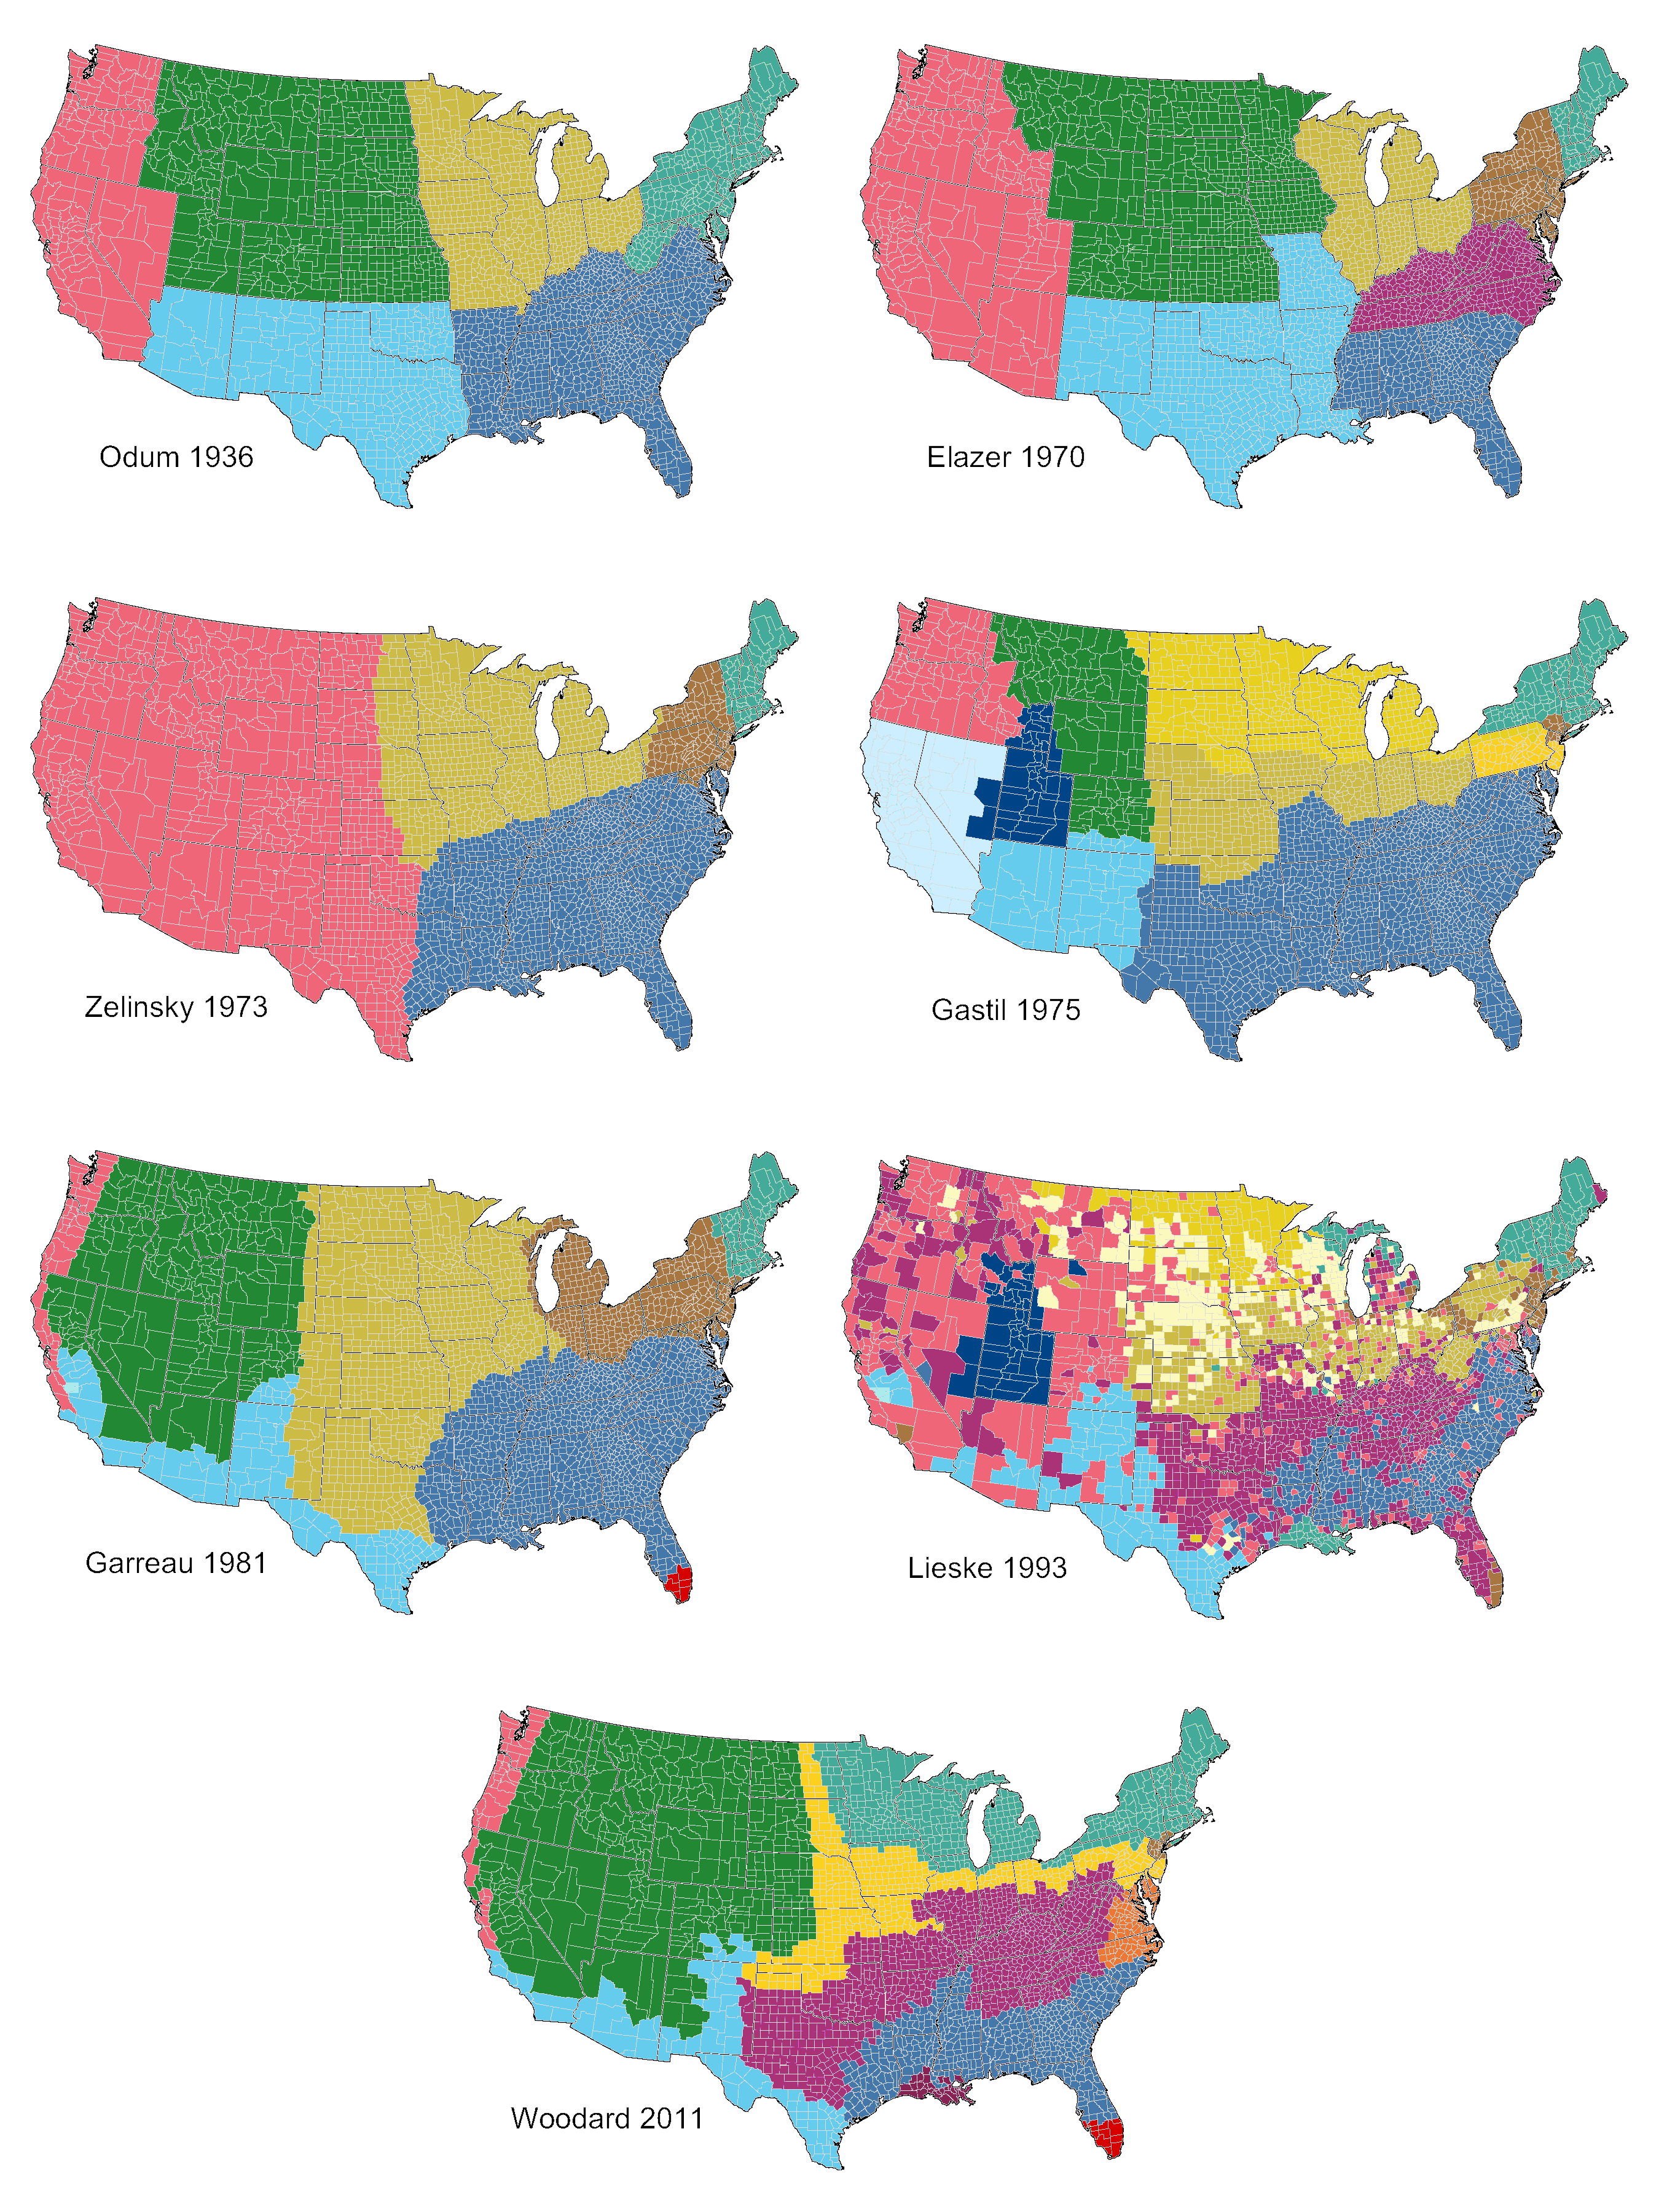
\includegraphics[width=1\textwidth]{litt_cultural_regions.png}
  \caption{Maps showing the primary American cultural regions as identified in eight
  previous studies at the county level
  \cite{OdumSouthernRegions1936,ElazarCitiesPrairie1970,ZelinskyCulturalGeography1992,GastilCulturalRegions1975,GarreauNineNations1996,LieskeRegionalSubcultures1993,WoodardAmericanNations2012}.}
  \label{fig:litt_cultural_regions}
\end{figure}

Given the subjectivity underlying these studies, the lack of agreement over the number
and location of American cultural regions (as illustrated in
\cref{fig:litt_cultural_regions}) is not surprising. Only a distinction between the
North and South, reflecting the Union-Confederacy border, and a distinction between the
East and West, reflecting the path of the Rocky Mountains, are common to these most
influential theories of American cultural
regions~\cite{OdumSouthernRegions1936,ElazarCitiesPrairie1970,ZelinskyCulturalGeography1992,GastilCulturalRegions1975,GarreauNineNations1996,FischerAlbionSeed1989,LieskeRegionalSubcultures1993,WoodardAmericanNations2012}.
Otherwise, between 4 and 12 primary cultural areas have been mapped, typically including
the
Northeast~\cite{OdumSouthernRegions1936,ElazarCitiesPrairie1970,ZelinskyCulturalGeography1992,GastilCulturalRegions1975,GarreauNineNations1996,FischerAlbionSeed1989,LieskeRegionalSubcultures1993},
the
South~\cite{OdumSouthernRegions1936,ElazarCitiesPrairie1970,ZelinskyCulturalGeography1992,GastilCulturalRegions1975,GarreauNineNations1996,FischerAlbionSeed1989,LieskeRegionalSubcultures1993,WoodardAmericanNations2012},
the
West~\cite{OdumSouthernRegions1936,ElazarCitiesPrairie1970,ZelinskyCulturalGeography1992,GastilCulturalRegions1975,GarreauNineNations1996,WoodardAmericanNations2012},
and the
Midwest~\cite{OdumSouthernRegions1936,ElazarCitiesPrairie1970,ZelinskyCulturalGeography1992,GastilCulturalRegions1975,GarreauNineNations1996}.

In large part, the debate over the geography of American cultural regions has been about
which types of cultural factors should be given precedence, and how these factors should
be combined. Crucially, these decisions have generally been left entirely to the
judgment of the analyst. Quantitative data from the census and elections have sometimes
been taken into consideration
(e.g.~\cite{ZelinskyCulturalGeography1992,GastilCulturalRegions1975,LieskeRegionalSubcultures1993,WoodardAmericanNations2012}),
but less often subjected to statistical analysis
(e.g.~\cite{LieskeRegionalSubcultures1993}), while the selection and weighting of these
factors has always been subjective. For example, religion and politics are undoubtedly
important cultural factors, but they can be measured in various ways, and it is unclear
how important they are relatively speaking and whether their importance varies across
the United States.

A basic question is therefore how can we infer general American cultural regions in an
objective way? In particular, how can we both identify a complete or at least
representative range of relevant cultural factors and somehow combine these factors in
so as to map American cultural regions? Defining such regions does not mean that they do
not contain internal variation or that they are separated by hard borders --- culture is
dynamic and complex and humans are highly mobile --- but that we can find areas where the
cultural practice and values of the people who live within that region are more similar
to each other than to those of people who live outside that region.

The goals of this work are therefore to address these issues, by (i) proposing a novel
method for discovering cultural regions by identifying regional patterns in topics of
conversation, and by then (ii) proposing a theory of American cultural regions derived
from the application of this method to a large corpus of geolocated social media data.


\section{Our approach}
Our starting premise is that cultural regions will necessarily be reflected by regional
variation in the topics that people choose to discuss in their everyday lives. If the
cultural geography of the US was broadly homogenous, we would expect topics of
conversation to be largely the same across the country, aside from different uses of
place names and other such relatively superficial and necessarily regionalized
vocabulary items. However, if  people from different regions exhibit distinct and
systematic cultural characteristics—for example, in politics, religion, music, sport,
fashion—as research on American cultural geography has consistently shown, then these
patterns of cultural variation will necessarily manifest themselves as patterns of
topical variation in the language used by people from these
regions~\cite{kramsch2014language}. For example, if hip hop music,  baseball, tattoos,
or some other cultural practice is especially popular in some part of the country, we
would expect more discussion on that topic in large samples of everyday language use
originating from that region, including on social media. Furthermore, previous works
show that cultural factors often show related regional patterns, owing presumably to
interrelationships between these different factors. For example, regional settlement
patterns can help explain differences in ethnicity and religion which can have long term
effects on voting patterns. Consequently, analyzing these regional topical patterns in
the aggregate can be used to infer broader cultural regions. Crucially, there is no need
to predefine what these topical patterns are or how much they matter: the topics
themselves and their relative importance can be inferred through the analysis of
everyday language as well. We therefore introduce an automated method for identifying
cultural regions based on the automated identification of patterns of regional variation
in topics of discussion in very large corpora of geotagged everyday language use. Our
method is especially intended to take advantage of the incredibly large amount of
geotagged social media data that online communication now provides us with for the first
time, although our method could be used to identify cultural regions within any area
based on any substantial source of regionalized everyday language use.

Specifically, to map modern American cultural regions, we identify regional patterns in
the topics that Americans tend to discuss on social media through a quantitative
analysis of ten thousand lexical items in over 3.3 billion geotagged tweets from across
the US, collected between 2015 and 2021. Large corpora of geotagged Twitter data have
been used frequently in computational
sociolinguistics~\cite{NguyenComputationalSociolinguistics2016}, and also in particular
to map patterns of dialect
variation~\cite{GrieveStatisticalMethod2011,EisensteinDiffusionLexical2014,GoncalvesCrowdsourcingDialect2014,HuangUnderstandingRegional2016,GrieveRegionalVariation2016,
DonosoDialectometricAnalysis2017,GoncalvesMappingAmericanization2018,AbitbolSocioeconomicDependencies2018,GrieveMappingLexical2019},
while others leveraged methods such as Latent Dirichlet Allocation to identify regional
topical patterns~\cite{KoyluUncoveringGeoSocial2018,FunknerGeographicalTopic2021}.
Despite this wealth of research that has used large corpora of social media to identify
regional patterns in language use, we are aware of no research that has used this type
of information to infer the location of general cultural regions.

Of course, social media or any other form of language can only provide a partial picture
of regional patterns in overall topics of discussion in a region. In general, big data
corpora generated from microblogging platforms certainly present a number of biases that we cited in \cref{sec:twitter_biases}. However, if cultural regions are real and pervasive, then
we should expect these regions to manifest themselves in any large sample of everyday
language that encompass a large proportion of the population, even if the specific
topics of interest vary across these different domains. Furthermore, right now, Twitter
is the only variety of geotagged natural language data available in sufficient amounts
to allow reliable automatic analyses, and is a very popular social media platform used
regularly by millions of people from across the US, mostly in interactive
contexts~\cite{AuxierSocialMedia2021}, serving as a perfect domain to apply our
data-driven approach for automatically mapping cultural regions.

Our main finding is that the modern US can be divided into five primary cultural areas,
each defined by its own topical patterns. We emphasize that this result stems from a
quantitative analysis in contrast to previous proposals based on more or less
informative (qualitative) approaches. Further, beyond the specific number of regions it
is most relevant to note that our method yields the list of words and topics that define
those regions, which highlights the differences in interests, habits and backgrounds
that distinguishes each cultural region from the others. Crucially, by means of a
dynamic analysis we show that cultural regions of the US are relatively stable over the
past few years, offering further evidence that cultural areas are real phenomena that
pervade American society.


The rest of the chapter is structured as follows.
\graffito{All code used for this work is hosted on GitHub \cite{LoufWordsuse2023}.}
The results of the work are first
introduced by a description of the dataset collection and pre-processing methodology.
Regional variations of words usage observed from this dataset are then explored, before
obtaining the principal dimensions of these variations. The main result of the work, the
cultural regions of the US and the main topics of discussion that define them, is then
presented in detail. The possibility of a variation with time of the results is then
explored. Finally, a discussion of the insights brought by the analysis and also of
where future works could build on it comes to conclude the chapter.


\section{Dataset}
We analyze 3.3 billion geotagged tweets from the contiguous US, posted from January
$1^\text{st}$, 2015 to December $31^\text{st}$, 2021. Importantly, we discard users
according to the criteria given in \cref{sec:method_users_select}. In our dataset, we
thus retain 17 million users. We clean the tweets' text and use the \ac{CLD} to
eliminate tweets written in a language other than English, following the process
described in \cref{sec:method_text_process}. We also remove tweets with a geotag that
did not allow for reliable assignment to our unit areas, which are the US counties and
county equivalents ($\SI{3108}{}$ in total), according to the criterion given in
\cref{tab:twitter_criteria}. Certainly, counties vary in both size and population but
most of them form a useful division sufficiently large to show a sizeable amount of
tweets and sufficiently small to allow for a careful delimitation of cultural areas
(states would be too big units whereas towns would be too small).

From the remaining tweets, we extract and count the tokens in their text, and assign
them to counties. Counties that accumulate fewer than \SI{50000}{} tokens are not taken
into account, leaving us with $N_c = \SI{2576}{}$ counties which define our sub-corpora.
We thus keep $\SI{83}{\percent}$ of the total number of counties. After this filtering,
the full dataset contains $9.1$ billion tokens. We subsequently convert the remaining
word forms to lowercase and aggregate the token counts on these forms. We then remove
all function words (like \textit{the, and}) and interjections (like \textit{um, oh}), and consider the
\SI{10000}{} most common remaining word forms. Note that this list of word forms emerges
from the data, and is not imposed by any previous topical or dialect classification.
All aggregated data generated by our Twitter data analyses as well as our list of
excluded words are available for download from a figshare repository
\cite{LoufWordCounts2023}

\begin{figure}[hpt!]
\centering
  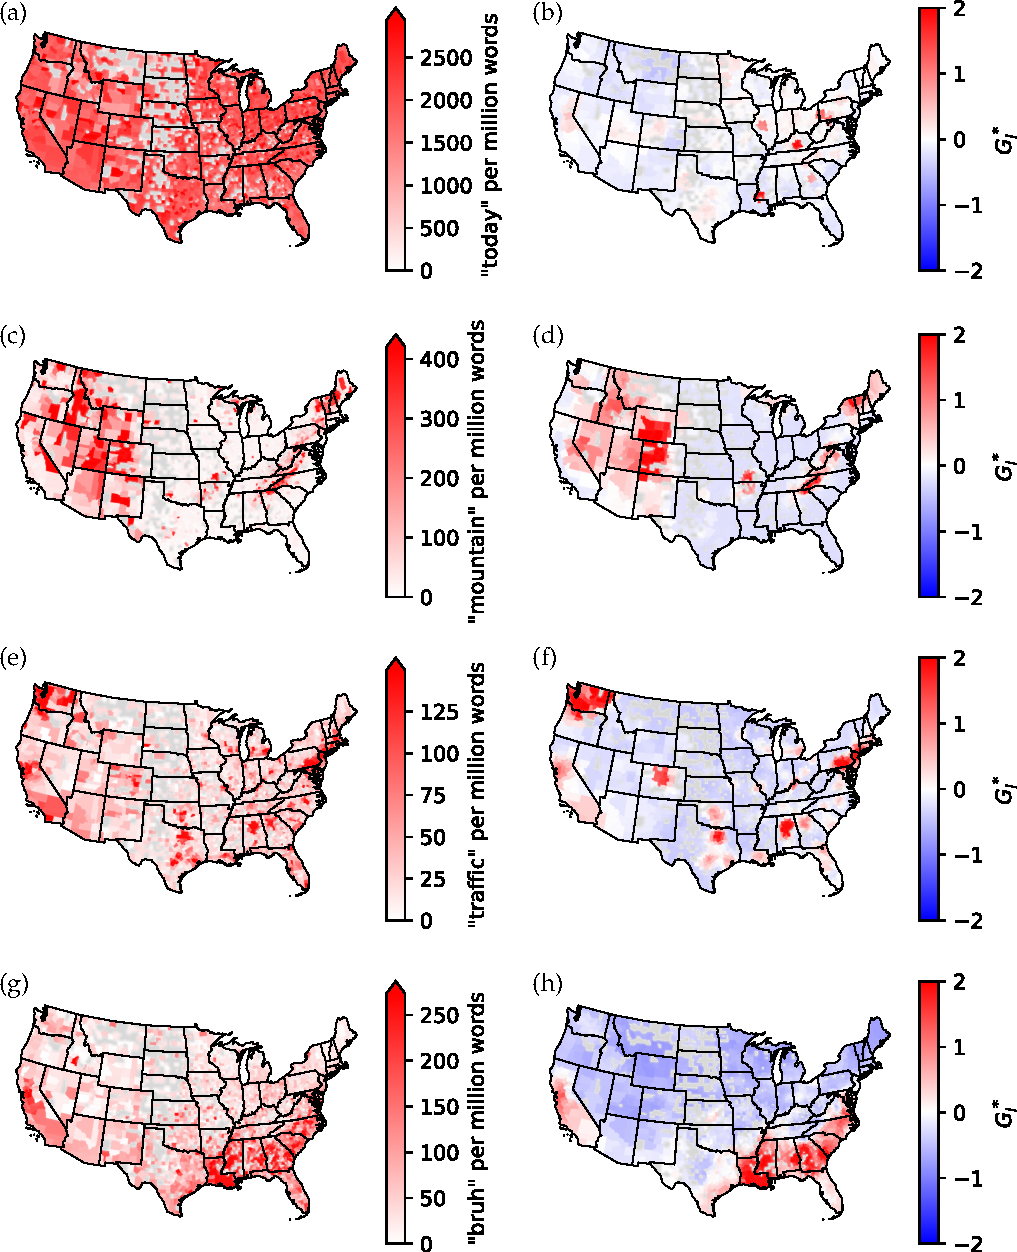
\includegraphics[width=1\textwidth]{example_words_maps.pdf}
  \caption{Maps showing the (a-c-e-g) relative frequency and (b-d-f-h) Getis-Ord
  $G_i^*$ z-score for the words \textit{today}, \textit{mountain}, \textit{traffic} and
  \textit{bruh}, respectively. One can note how the latter metric enables to reveal word
  usage hotspots, smoothing out the raw noisy signal from the data.}
  \label{fig:example_words_maps}
\end{figure}


\section{Measuring regional variation}
We then measure and map the relative frequencies $f_{c, w}$ for every word $w$ in every
county $c$. We illustrate our raw results by plotting in \cref{fig:example_words_maps}
the relative frequency in each county of four representative words: (a) \textit{today},
(c) \textit{mountain}, (e) \textit{traffic} and (g) \textit{bruh} (cells that appear
greyed out do not reach a minimum number of tweets as explained in the paragraph above).
In the first case, \textit{today} appears at relatively stable rates in most of the
counties, as expected. Alternatively, \textit{mountain} is a regionally-dependent word
as clearly seen. The item \textit{traffic} appears more frequently in urban areas.
Finally, \textit{bruh} is an African-American English variant that appears to be
especially common in southern counties, where there are large African-American
populations.

A word of caution is now required. A relative frequency map alone is not able to fully
reveal regional variations due to the wide range of different factors besides regional
variation that affect word use and add noise to the signal. To extract the underlying
regional signal from each word map, we conduct a multivariate spatial analysis
\cite{GrieveStatisticalMethod2011,GrieveRegionalVariation2016} of the relative
frequencies of our \SI{10000}{} word forms. In order to identify geographical hotspots
in the usage of each word (\cref{fig:example_words_maps}), we compute Getis-Ord's
z-scores ($G_i^*$ \cite{OrdLocalSpatial1995}) for each county $c$ and word $w$, which
are defined as:
\begin{equation}
\label{eq:Gi_star}
  G_{c, w}^* = \frac{
      \sum_{c'} W_{c, c'} (f_{c', w} - \bar{f_w})
    }{
      \sigma_w \sqrt{\frac{
        N_c \sum_{c'} W_{c, c'}^2
          - \left( \sum_{c'} W_{c, c'} \right)^2
        }{
          N_c - 1
        }
      }
    },
\end{equation}
with $\bar{f_w}$ the average frequency of $w$ over the whole dataset, $\sigma_w$ the
standard deviation in $w$'s frequencies, and $W_{c, c'}$ are the elements of a proximity
matrix, which we take as equal to $1$ if $c' = c$ or $c'$ belonging to $c$'s 10 nearest
neighbors, and equal to $0$ otherwise.

The metric given by \cref{eq:Gi_star} ultimately diminishes spurious data variation and
smooths spatial patterns, allowing us to discern a regional pattern in a word's usage.
In \cref{fig:example_words_maps}(b), (d), (f) and (h) we show, respectively, the $G_i^*$
z-scores for the previous words \textit{today}, \textit{mountain}, \textit{traffic} and
\textit{bruh}. White, light blue or light red counties do not depart significantly from
an average utilization, whereas a bright red or blue respectively mean that the word is
relatively frequently or infrequently used in that region. Since \textit{today} is a
rather generic word, we do not find any strong regional pattern, whereas the others do.
The usage hotspots of \textit{mountain} display the main mountain ranges of the country.
While the map for \textit{traffic} is correlated with large urban areas (and can be
interpreted as a topical word), the dialect word \textit{bruh} seems to be significantly
more used in counties pertaining to the Deep South. We see here that different
attributes that define a culture (interests, behavior, dialect) are captured within our
scheme and, notably, are treated on equal footing.


\section{Obtaining the principal dimensions of regional variation}
The $G_i^*$ distributions for all \SI{10000}{} top words by usage thus hold valuable
information. However, a considerable part of this information can be analyzed more
efficiently, since some words may belong to the same semantic field (\textit{mountain}
and \textit{peak}) or characterize the same particular dialect (\textit{bruh} and
\textit{aight}). Furthermore, a few variations may simply be uninformative noise,
intrinsic to real individuals' behaviors, but also potentially resulting from an
imperfect filtering of Twitter data, as aforementioned. The most important dimensions of
regional lexical variation are then found by subjecting the hotspot maps for the
complete set of words to a \ac{PCA}
\cite{LieskeRegionalSubcultures1993,WoldPrincipalComponent1987}. Another possible
approach would have consisted in performing topic modelling, for instance by ways of a
latent Dirichlet allocation on the word frequency matrix, to then infer a distribution
of topics for every county. It is however more computationally intensive, and poses the
questions of the selection of the number of topics, their interpretability and their
internal coherence \cite{ArunFindingNatural2010,HasanNormalizedApproach2021}. In a case
like ours where documents are so large (aggregating all tweets in a county), it is far
from obvious to select a number of topics such that there is little overlap between
them, and to know that these topics are actually representative of the dataset as a
whole. This is much more clear when selecting components in \ac{PCA}, as we show
below.

From the $N_w = \SI{10000}{}$ dimensions of our dataset, we thus project to a \ac{PC}
space of $N_{\text{PC}} = 326$ dimensions. It turns out that these 326 components
explain 92~\% of the observed variance (see \cref{fig:whole_data_decomp}(f)). We do not
set this number of components arbitrarily, by choosing one directly or by setting a
percentage of variance we wish to explain using these components. Instead, we use the
broken-stick rule to fix the number of components
\cite{FrontierEtudeDecroissance1976,JacksonStoppingRules1993}. This heuristic compares
the decrease of the variance explained by each successive component to the one expected
from a random partition of the whole variance in $N_w$ parts. Components, sorted by
decreasing explained variance, are kept until they do not explain more variance than
their corresponding random part would. With this method, we do not make any assumption
about the amount of variance in our data that is simply due to random fluctuations.

We show the projected data along the first four \acp{PC} in
\cref{fig:whole_data_decomp}(a-d), which displays a neat visualization of the spatial
patterns. The map for each dimension shows two opposing regions (red and blue) which can
be linked to their characteristic words, the ones with the highest (positive, in red)
and lowest (negative, in blue) loading. For an illustration, in
\cref{fig:whole_data_decomp}(e) we show in a word cloud the most characteristic words
for each of the two regions in \cref{fig:whole_data_decomp}(b), which corresponds to the
second component.

\begin{figure}[ht!]
\centering
  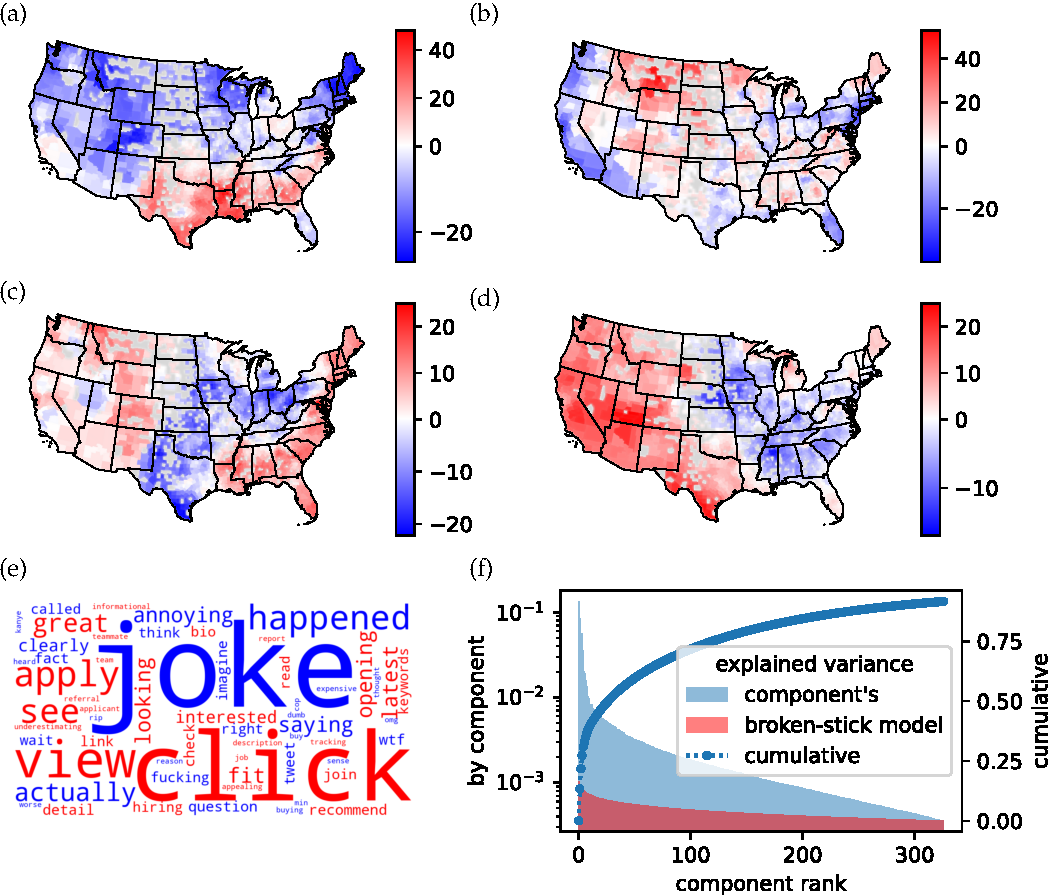
\includegraphics[width=1\textwidth]{whole_data_decomp.pdf}
  \caption{Result of the \ac{PCA} carried out on our whole dataset. (a-d) Four maps show
  the projection of the data along the first four components, highlighting regional
  lexical variations. Note that the scale on the divergent color scales are not
  symmetrical around zero in order to utilize the full range of colors of the color map.
  (e) Word cloud showing the words with the strongest positive (red) and negative (blue)
  loadings for the second component, with each word's font size depending on its
  loading's absolute value. (f) Explained variance of the \acp{PC} compared to the
  broken-stick model on a logarithmic scale, which shows how the number of components to
  keep is selected at the first intersection of the two curves. The cumulative
  proportion of the variance explained by the components is also plotted, showing that
  our dimension reduction explains around 92\% of the observed variance. The first four
  components shown in panels (a-d) capture alone 31\% of the variance.}
  \label{fig:whole_data_decomp}
\end{figure}


\section{Inferring cultural regions}
We are now in a position to generate a single overall taxonomy of American cultural
regions by clustering together counties with similar lexical signature. To do so, we
subject the previous \ac{PC} maps to a hierarchical clustering, using the Euclidean
distance and the Ward variance minimization algorithm \cite{EverittClusterAnalysis2011}.
This is how we define the cultural regions from our corpus, as depicted in
\cref{fig:whole_data_clust}. From the dendrogram and the evolution of the average
silhouette score for different levels of clustering, we select a meaningful number of
clusters $n_{\text{clusters}}$ \cite{RousseeuwSilhouettesGraphical1987}. The
hierarchical nature of the clustering is useful to see how regions are grouped together
at different levels of clustering, indicating which regions are closer together.
Importantly, applying hierarchical clustering to the principal dimensions of variation
of the data obtained through \ac{PCA} allows us to focus on the main regional
patterns of variation. Applying the algorithm directly to the $\SI{10000}{}$-word
distance matrix would yield highly noisy results.

We plot the main divisions in \cref{fig:whole_data_clust}(a). This is the main result of
the chapter. In the map, we present the division into five clusters since it is one of the
two best options as characterized by the Silhouette score analysis in
\cref{fig:whole_data_clust}(b), and at a clear-cut on the dendrogram in
\cref{fig:whole_data_clust}(d). The optimal choices correspond to the two significant
drops in the score: the first (second) corresponds to a cluster number equal to 2 (5). 

Indeed, the dendrogram in \cref{fig:whole_data_clust}(d) shows that the counties can be
initially classified into two large-scale subgroups representing a North vs South
divide. The North is then further fragmented into the clusters 2, 3 and 4 shown in
\cref{fig:whole_data_clust}(a), whereas the South group splits into the clusters 1 and
5. For the most part, our map in \cref{fig:whole_data_clust}(a) is consistent with
standard theories of American cultural regions, with all five of our regions finding
analogs in existing systems. Yet, taken as a whole our clusters do not match any
previous system and reveal non-contiguous culture regions such as the clusters 3 and 4.
Moreover, in contrast to previous proposals our results have the advantage of being
data-driven, based on variation in the topics people care to discuss as opposed to
factors selected by hand by the researcher (and consequently subjected to many more,
uncontrolled biases than our Twitter data).

Further, to be able to better interpret the obtained regions, it is insightful to know
which words characterize each cluster the most. To infer them, we start by taking the
center of each cluster in words-$G_i^*$-space. Hence, for each cluster we take the
average $G_i^*$ score over its counties for all words. From these $n_{\text{clusters}}$
vectors of $N_w$ elements, we calculate the minimum absolute difference between each
cluster center's word's score and the ones of all other clusters, i.e., we take the
distance to the closest cluster's center along the word's dimension. More formally, we
define the specificity $S_{C, w}$ of word $w$ for cluster $C$ as:
\begin{equation}
\label{eq:spec}
  S_{C, w} = \min_{C' \; \in \; \mathcal{C} \setminus C} \left(
  \frac{1}{N_C} \sum_{c \; \in \; C} G_{c, w}^*
    - \frac{1}{N_{C'}} \sum_{c \; \in \; C'} G_{c, w}^*
  \right)^2 ,
\end{equation}
where $\mathcal{C}$ denotes the set of clusters, $N_C$ the number of counties belonging
to cluster $C$, and $G_{c, w}^*$ the $G_i^*$ score of word $w$ in county $c$. For each
cluster $C$, we thus define the most characteristic words as the ones with highest
$S_{C, w}$ values. In the case of the division in five clusters, the top 5 most
characteristic words per cluster are shown in \cref{fig:whole_data_clust}(c), according
to the specificity metric defined in \cref{eq:spec}. In all cases, the five cultural
regions are linked to clear and distinct topical patterns (see the Supplementary
Information for a more exhaustive list). We stress that these characteristic words are
automatically identified based on the quantitative analysis presented above. Notably,
for each cluster we see three basic type of lexical patterns. 

\begin{figure}[ht!]
\centering
  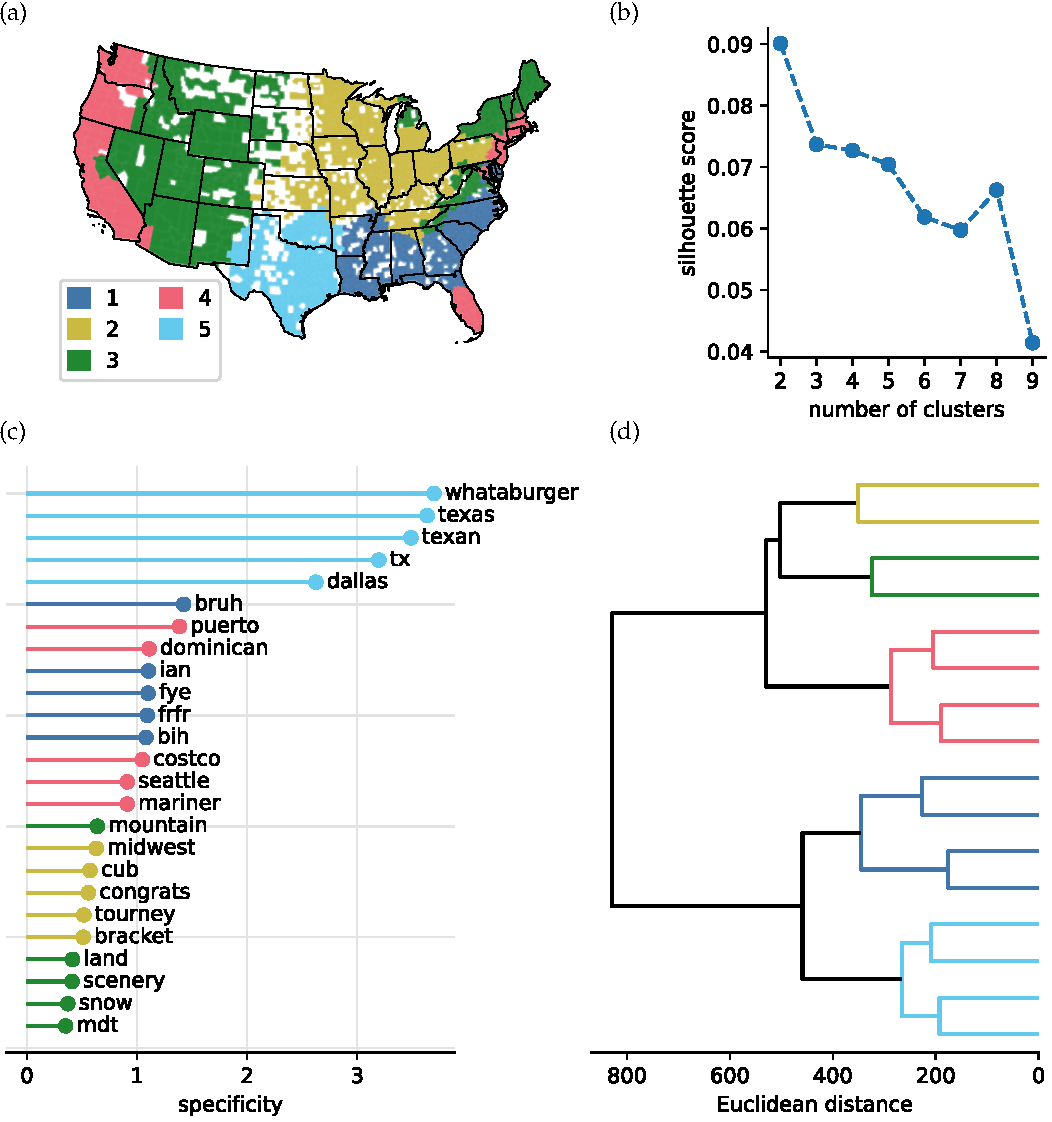
\includegraphics[width=1\textwidth]{whole_data_clust.pdf}
  \caption{Cultural regions obtained from our whole dataset. (a) Map of the five
  clusters obtained through hierarchical clustering, selected from a high value of (b)
  the mean Silhouette score. A significant drop of the Silhouette score after 5 levels
  indicates that further splitting counties in more region does not yield coherent
  cultural regions. (c) Five most specific words for the five clusters shown in (a),
  along with their specificity values. (d) The dendrogram allows seeing which clusters
  are first joined if going to a higher level of clustering, and thus which ones are
  closer together. It clearly shows that the strongest division is the one between the
  North and the Southeast (excluding Florida) with further splittings as the cluster
  distance increases.}
  \label{fig:whole_data_clust}
\end{figure}  

First, we see words associated directly with those locations, most commonly the names of
cities, states, and sports teams. This is basic evidence that the method works: we would
expect these words to be associated with the cultural regions that contain them.
However, these results also reflect how often people from different cities and states
refer to each other. For example, the fifth cluster which is centered on Texas also
includes Oklahoma, which contributes various place names to the list of words most
strongly associated with this region. This means not only that people in Texas and
Oklahoma talk more about place names in their own states, as would be expected, but that
they talk more about place names in each other's states. This is one type of regional
topical patterns that our approach draws to identify cultural regions.

Second, we observe words connected with non-regional topics, which nonetheless show
regional differences. In this case, our approach can be seen as discovering topical
patterns and by extension cultural patterns that distinguish between different regions
of the US. For example, cluster 2 is strongly associated with the discussion of a range
of American sports, as well as the names of the states that fall within this region.
Although we would expect that a region centered around the Midwest would be associated
with the names for Midwestern states, their preoccupation with the discussion of sports
on Twitter is not so easy to predict. 

Third, we find words that are dialect items, i.e., alternative ways of referring to a
given concept. This type pattern is especially apparent for cluster 1, which aligns
closely with the region of African American population density and is therefore
associated with numerous lexical items from African-American English (e.g. \textit{bruh,
lawd, turnt}). Although dialectologists do not usually focus on the frequencies of
individual words, this results is to be expected: dialect regions, which can be seen as
a type of cultural region, have been found to generally align with broader cultural
regions~\cite{GrieveRegionalVariation2016}.

We can now examine each of the five cultural regions we have identified in turn and
consider what the words that are mostly strongly associated with each tell us about the
culture of that region, as well as the factors that drive cultural variation in the US
more generally. 

The first cluster [blue in \cref{fig:whole_data_clust}(a)], which identifies a
southeastern region, largely reflects African American culture, as can be predicted
based on the close correlation between our map and the distribution of counties with
relatively large African American populations. Most notably, tweets from
the South are more likely to contain words related to African American culture,
including, for example, cuisine (e.g. \textit{grits, cookout}), fashion (e.g.
\textit{braids, dreads}), and music (e.g. \textit{rappers, rapping}). As noted above,
this cluster is also strongly characterized by many vocabulary items associated with
African American English, especially for referring to people (e.g. \textit{bruh, dawg}),
as well as many acronyms (e.g. \textit{frfr, stg}). Place names associated most strongly
with this cluster primarily include southern states (e.g. \textit{Georgia, Carolina}),
despite the fact that, in general, references to place names are relatively rare
compared to other clusters.

The second cluster [yellow in \cref{fig:whole_data_clust}(a)] has its core in the
Midwest and is clearly characterized by more frequent references to sports. American
team sports especially stand out, with 40 words of the top 50 most strongly associated
with this cluster being directly linked to this topic. In particular, these are words
associated with basketball (e.g. \textit{basketball, rebound}) and baseball (e.g.
\textit{baseball, innings}), although football, wrestling, and cheering are also
referenced, as well as various more generic sporting terms (e.g. \textit{teams,
tourney}). Similarly, many place names are associated with local sports teams (e.g.
\textit{Cubs, Chiefs}), although various state names are also strongly associated with
this cluster (e.g. \textit{Ohio, Illinois}), as well as the word \textit{Midwest}
itself.  A smaller number of lexical items are also associated with school (e.g.
\textit{locker, choir}). Overall, this cluster therefore shows that sports is a central
part of this region. 

The third cluster [green in \cref{fig:whole_data_clust}(a)] can be identified with a
discontinuous region that mostly aligns with rural areas of the US, as well as areas
that focus on outdoor activities, especially in mountainous regions (e.g., the Rocky or
Appalachian Mountains). This cluster is relatively hard to interpret topically, in part
because, unlike the other regions, it is characterized by the relative infrequent use of
a number of words. In terms of words that are relatively common in this region, the
clearest pattern is a relatively large number of words associated with nature (e.g.
\textit{mountains, tree}), weather (e.g. \textit{snow, seasonal}), and outdoor
activities (e.g. \textit{adventures, trail}). Clearly, people in this region tend to
focus more of their natural surroundings. In addition, there are a number of words
related to work (e.g. \textit{hiring, jobs}), as well as a numerous place names (e.g.
\textit{Colorado, Montana}) that are strongly associated with this region. In terms of
words that are uncommon within the cluster, there exist many verbs, especially verbs
associated with human actions like communication (e.g. \textit{said, told}), thought
(e.g. \textit{understand, confused}), and physical actions (e.g. \textit{put, hit}),
which implies overall less focus on the individual. This region is also associated with
relatively infrequent use of a wide range of negative words (e.g. \textit{wrong, bad}),
which largely hints at a more positive outlook.  

The fourth cluster [red in \cref{fig:whole_data_clust}(a)] also identifies a
discontinuous region that primarily encompasses large urban areas in the coasts
(Northeast and West). Unsurprisingly, this region is characterized by a wide range of
words associated with more urban life (e.g. \textit{homeless, traffic}), especially
terms related to different nationalities and immigration (e.g. \textit{Latino, Asian}).
We also find a relatively large number of place names (e.g. \textit{California, NYC}).
Strikingly, this cluster is associated with a very large number of words with negative
connotations, including relating to violence (e.g. \textit{violence, attack}), danger
(e.g. \textit{dangerous, crime}), cursing (e.g. \textit{asshole, fucking}), political
unrest (e.g. \textit{protests, indicted}), racism (e.g. \textit{Nazi, supremacist}), and
general negative adjectives (e.g. \textit{disgusting, abusive}). Quite generally, people
from this cluster are more likely to discuss negative topics than other parts of the US,
at least on social media. Taken together, the third and fourth clusters suggest an
opposition in the culture of more rural and urban areas in the US, which appear to
engage in more positive and negative discourse respectively~\cite{vanderbeck2003young}. 

Finally, the fifth cluster [cyan in \cref{fig:whole_data_clust}(a)], which is centered
around South Central States, especially Texas and Oklahoma, is characterized by frequent
reference to place names, relative to the other clusters, especially in these two
states, as has already been noted. For example, the first five most strongly associated
words are \textit{Whataburger} (a fast food chain from Texas), followed by
\textit{Texas, TX, Texan, and Dallas}. This not only shows that people in this region
tend to discuss place more on Twitter, but implies that this cultural region is
characterized by a relatively high amount of local pride. Correspondingly, this region
is also associated with a relatively large number of dialect terms, both of Anglo (e.g.
\textit{yalls, fixing}) and Hispanic (e.g. \textit{queso, taco}) origins, reflecting the
diverse makeup of this region.

Given the lack of consensus in previous research, our results can help resolve
long-standing debates relating to the distribution of American cultural regions. We find
that the division between the Southeast and the rest of the US is the strongest. This
result attests to the importance of the cultural divide between White and Black America
and between the North and the South. Although all previous major theories of American
cultural regions has identified a distinction between the North and the South, our
southern region is especially similar to relatively recent theories, which identify a
southern region that closely aligns with the part of the south with an especially high
proportion of African Americans
\cite{LieskeRegionalSubcultures1993,WoodardAmericanNations2012}. Another key finding
that emerged from our analysis is a broad opposition between coastal and internal areas,
which has not previously been identified as important sources of distinction of American
cultural regions
\cite{OdumSouthernRegions1936,ElazarCitiesPrairie1970,ZelinskyCulturalGeography1992,GastilCulturalRegions1975,GarreauNineNations1996,FischerAlbionSeed1989,LieskeRegionalSubcultures1993,WoodardAmericanNations2012}
but reflects a modern political trend of undeniable significance
\cite{GelmanRedState2009} that is currently reconfiguring the nation. The discontinuous
nature of these regions, which is not required by our definition of a cultural region,
is also notable. It demonstrates how patterns in American culture can be distributed
across very wide areas, reflecting complex patterns in physical and human geography, and
the underlying complexity and dynamic nature of American society. This result is broadly
in line with other recent theories of American cultural regions which have also
identified discontinuous cultural regions
\cite{LieskeRegionalSubcultures1993,WoodardAmericanNations2012}.

Our analysis is further useful for understanding the relationship between these regions.
It divides the South into two regions, splitting Texas off from the rest of the
Southeast, and splits the Midwest off from the rest of the North, divided into
discontinuous countryside/coastal regions, rather than contiguous cultural regions.
However, on the question of the number of primary American cultural regions, we can only
safely say that with our data and methodology, at least 5 distinct regions can be
discerned. We do not see it here, but we still cannot discard recent theories that claim
that America is fundamentally far more culturally fragmented
\cite{GarreauNineNations1996,LieskeRegionalSubcultures1993,WoodardAmericanNations2012}.


\section{Temporal aspect of the results}
Given the success of our analysis, it would be interesting to see how the cultural
regions found in \cref{fig:whole_data_clust} change with time, as has been done in other
research analyzing diachronic corpora
\cite{BochkarevAverageWord2015,BentleyBooksAverage2014,KarjusQuantifyingDynamics2020,MomeniModelingEvolution2018,AlshaabiStorywranglerMassive2021}.
Although we would not expect significant changes due to the short timescale imposed by
our Twitter dataset, we can still carry out a diachronic study to validate the very
existence and meaningfulness of the cultural regions. To do so, we split our corpus into
three datasets corresponding to different year ranges: 2015-2016, 2017-2018 and
2019-2021. These periods have a similar amount of tokens and can be then subjected to
comparison. We show their maps in
\cref{fig:evol_comp1_dists}(a-c). We obtain similar patterns, despite the variety of
topics and forms employed on Twitter along the years and the heuristic nature of the
clustering method that introduces a small amount of noise in the results. The
North-South division is stable over time with small variations that can be due to either
fluctuations or incipient structural changes. The latter cannot be conclusive due to the
short time period considered in this work.

\begin{figure}[ht!]
\centering
  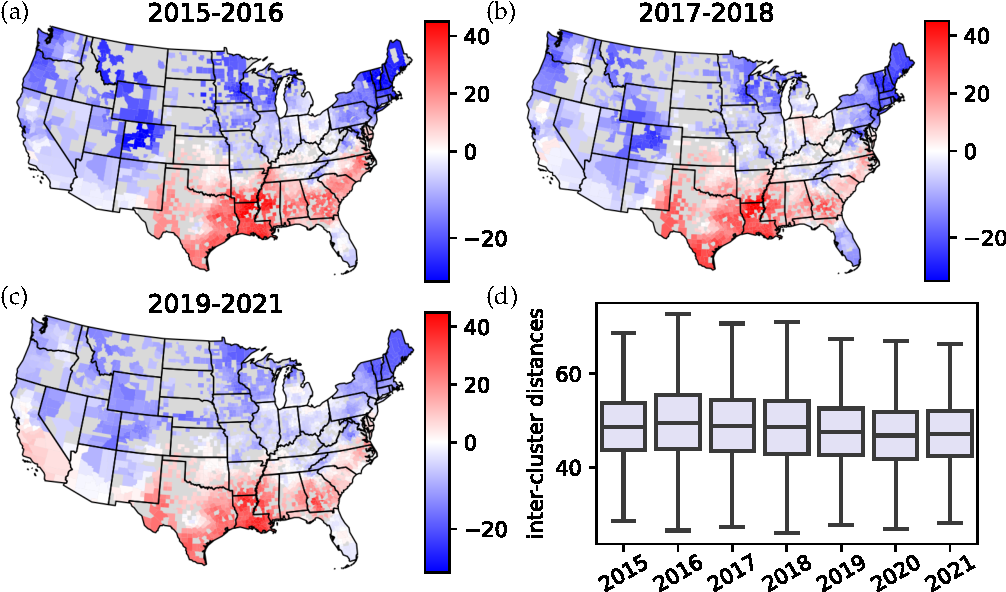
\includegraphics[width=1\textwidth]{evol_comp1_dists.pdf}
  \caption{Effect of temporal segmentation for the data on the obtained divisions. (a-c)
  Maps of the data projected along the first \ac{PC} obtained for the years 2015-2016,
  2017-2018 and 2019-2021, respectively. Apart from slight variations in California and
  Florida, the first component translates the same division between the Southeast and
  the rest of the US. Note that the scale on the divergent color scales are not
  symmetrical around zero in order to utilize the full range of colors of the color map.
  (d) Evolution of the distributions of inter-cluster distances along the years spanned
  by our dataset. The box plots show the median, first and third quartile, and the
  boundaries of the whiskers are within the 1.5 interquartile range value. We use the
  cluster assignment obtained with the whole dataset and measure the Euclidean distance
  in $G_i^*$ space between counties belonging to different counties. The distribution is
  thus shown to vary little from year to year,  which demonstrates the stability of the
  two-way division we found.}
  \label{fig:evol_comp1_dists}
\end{figure}

Next, we take the hierarchical clustering in \cref{fig:whole_data_clust}(d) and select
the county-to-cluster assignment corresponding to the highest level of the hierarchy.
This is represented by the two-way division between North and South. For each year in
our dataset, we then measure the pairwise distances between counties belonging to both
clusters. The distances are calculated as Euclidean distances between rows of the matrix
$G_{c, w}^*$ (see \cref{eq:Gi_star}). We thus obtain the evolution with time of the
inter-cluster distances distribution as shown in \cref{fig:evol_comp1_dists}(d). The box
plots demonstrate that (i) the median distance is roughly constant over the years, and
(ii) the distance distribution shows little variation. Both findings suggest that the
detected cultural regions are no artifact of the method, but a genuine data structure
that exists within our corpus.
% mention clustering can yield any result, there will always be clusters detected, but to have stable picture shows 
% But on the short timescale our dataset spans, or even of Twitter's own lifespan, we
% cannot expect to be able to observe significant cultural changes. 


\section{Discussion}
Overall, our analysis has therefore identified regional patterns of lexical variation of
clear cultural importance. Furthermore, the themes associated with each of these
patterns provide a new perspective on American cultural geography. For example, although
our analysis has confirmed that factors such as ethnicity and religion are important for
defining American cultural regions, we found substantial variation in the relevance of
these factors across the US. Our analysis has also identified other subtler cultural
patterns --- such as a focus on social interaction, the outdoors, family, and
leisure --- which have been overlooked in previous research, in part because they cannot
be easily studied through the analysis of traditional sources of secondary data. Our
method has therefore not only allowed us to map cultural regions, but it has also
allowed us to identify cultural factors that are important for defining these regions,
at least in this communicative context, providing a foundation for a more complete
picture of the American cultural landscape.

Clearly, this study has only analyzed one genre of American English. The specific topical
patterns on Twitter would not be exactly replicated in other genres, especially given
the communicative purpose and user base associated with microblogging platforms.
Nevertheless, assuming that American cultural regions are important and pervasive
forces, similar regional patterns should be reflected across all popular genres. This issue
could be further clarified when more richly annotated natural language data becomes
available in a near future. Our methods, however, will remain valid for any such
dataset. Crucially, we expect that our main idea of inferring cultural regions and the
topics defining them from people's speech will be applicable to any big data resource
with linguistic value.


\end{document}
